\chapter{Spectral Energy Distribution Analysis}

\section{SED Fitting Method}

In order to determine a dust mass, we use the IDL package MPFIT \citep{markwardt2009} which utilizes the Levenberg-Marquardt algorithm.  The Levenberg-Marquardt algorithm is will use a combination of two minimization techniques (the steepest descent method and the Newton-Raphson Method) to determine the parameter combination that will lead to a minimum in the $\chi^2$ space \citep{burden2001}.  The algorithm begins by implementing the steepest descent method in order to traverse the $\chi^2$ space in the direction of the steepest gradient.  As the set of solutions approaches a minimum, it will use the Newton-Raphson method to locate best set of parameters by finding where the derivative at that point is closest to zero \citep{gavin2013}.  

In order for MPFIT to provide the most accurate fit, we establish a reasonable error for each of our data points, and determine a realistic set of starting points for the fitting.  The variance for our SCUBA-2 data is determined by equation \ref{eq:sc2noi} such that $\sigma_{obs}$ is the noise determined by MAKEMAP, $\sigma_{rms,sky}$ is the RMS of the sky, and $\sigma_{calib}$ is the calibration uncertainties where the scaling factor is shown in table \ref{tab:calib_fac}.

\begin{equation}\label{eq:sc2noi}
  \sigma^2 = \sigma_{obs}^2 + \sigma_{rms,sky}^2 + \sigma_{calib}^2
\end{equation}

\begin{deluxetable}{cc}
%  \tabletypesize{\footnotesize}
  \tablecolumns{2}
  \tablewidth{0pt}
  \tablecaption{Calibration Factors for SCUBA-2 and KINGFISH Observations}
  \label{tab:calib_fac}
  \tablehead{\colhead{Observation} & \colhead{Scaling Factor}}
    \startdata
      100$\mu$m & 0.03 \\
      160$\mu$m & 0.05 \\
      250$\mu$m & 0.07 \\
      350$\mu$m & 0.07 \\
      450$\mu$m & 0.12 \\
      500$\mu$m & 0.07 \\
      850$\mu$m & 0.08 \\
    \enddata
\end{deluxetable} 

The variance for the KINGFISH data are determined in a similar fashion shown in equation \ref{eq:kinnoi}, however the observation error is excluded since the reported variance in the filtered images are reflective of the fake source image used and not of the KINGFISH data set.

\begin{equation}\label{eq:kinnoi}
  \sigma^2 = \sigma_{rms,sky}^2 + \sigma_{calib}^2
\end{equation}

The nature of the Levinberg-Marquardt method leaves the solution vulnerable to converge at a local minimum rather than converging at the global minimum.  This is remedied by selecting reasonable initial conditions.  The initial conditions we used were 20K for the temperature, a dust emissivity index of 2, and a mass determined by equation \ref{eq:mass} using the flux from the 250$\mu$m emission and our initial temperature and dust emissivity values.  

\begin{equation}\label{eq:mass}
  \begin{split}
    M & = \frac{D^2 \: I_{250}}{\kappa_{\nu,0} \:  B_{250}\left(20\right)} \left(\frac{\nu}{\nu_0} \right)^{-\left(2+3\right)} \\
      & = 2.24 \times 10^5 \: I_{250} \; \left[M_\odot\right]
  \end{split}
\end{equation}

\section{Fitting the Spectral Energy Distribution}

The fitting procedure was carried out in two different ways on a modified blackbody equation, equation \ref{eq:mod_sed}. 

\begin{equation}\label{eq:mod_sed}
  S_\nu\left(T\right) = \frac{M\:\kappa_{\nu,0}}{D^2}\left(\frac{\nu}{\nu_0}\right)^{\beta+3} B_\nu\left(T\right)
\end{equation}

One of the two methods is fitting an SED to each individual pixel in order to generate a set of parameter maps, and the second is by totaling the flux of each of the selected regions shown in figure \ref{fig:regions} to maximize the signal to noise ratio in order to generate a more precise set of parameters.  For both of the fitting methods the mass, $M$, and temperature, $T$, are set as free parameters, but the treatment of the dust emissivity index, $\beta$, required special treatment for each of the methods.  The distance, D, has been set to 9.4 Mpc \citep{?}, and the reference opacity, $\kappa_{\nu,0}$, was tested using"" \citep{lianddrane} and "" \citep{planck20??}

\subsection{Pixel SED Fits}

In order to generate a parameter map of NGC3627, each individual pixel has it's own SED determined from the available wavelengths described in the observations chapter.  The treatment of the dust emissivity index is performed by fixing it at $\beta=1.8$ for the Planck opacity model such that the opacity is $\kappa_{300\mu m,0}=1.0$ m$^2$kg$^{-1}$ \citep{planck252011} and $\beta=2.0$ for the Li and Draine opacity model where the opacity is $\kappa_{300\mu m,0}=0.2665$ m$^2$km$^{-1}$ \citep{li2001}.  A third fit is performed where the emissivity index is allowed to vary as a free parameter.  While the emissivity index is allowed to vary, the opacity being used is the Planck model.  This is justifiable because the opacity will not effect the shape of the SED, only the its normalizing value.  In the case of our fits, it is the mass that acts as the normalizing consant, so increasing or decreasing the opacity will yeild the opposite effect in the mass.  The inverse proportionality can be seen in equation \ref{eq:mass}.  The resulting parameter maps of the fits are shown in figure \ref{fig:param_fits}. The numerical values from fitting each model are shown in tables \ref{tab:beta_1}, \ref{tab:beta_2}, \ref{tab:beta_f} where each region correspondes to the regions labeled in figure \ref{fig:regions}.

\begin{figure}
  \centering
  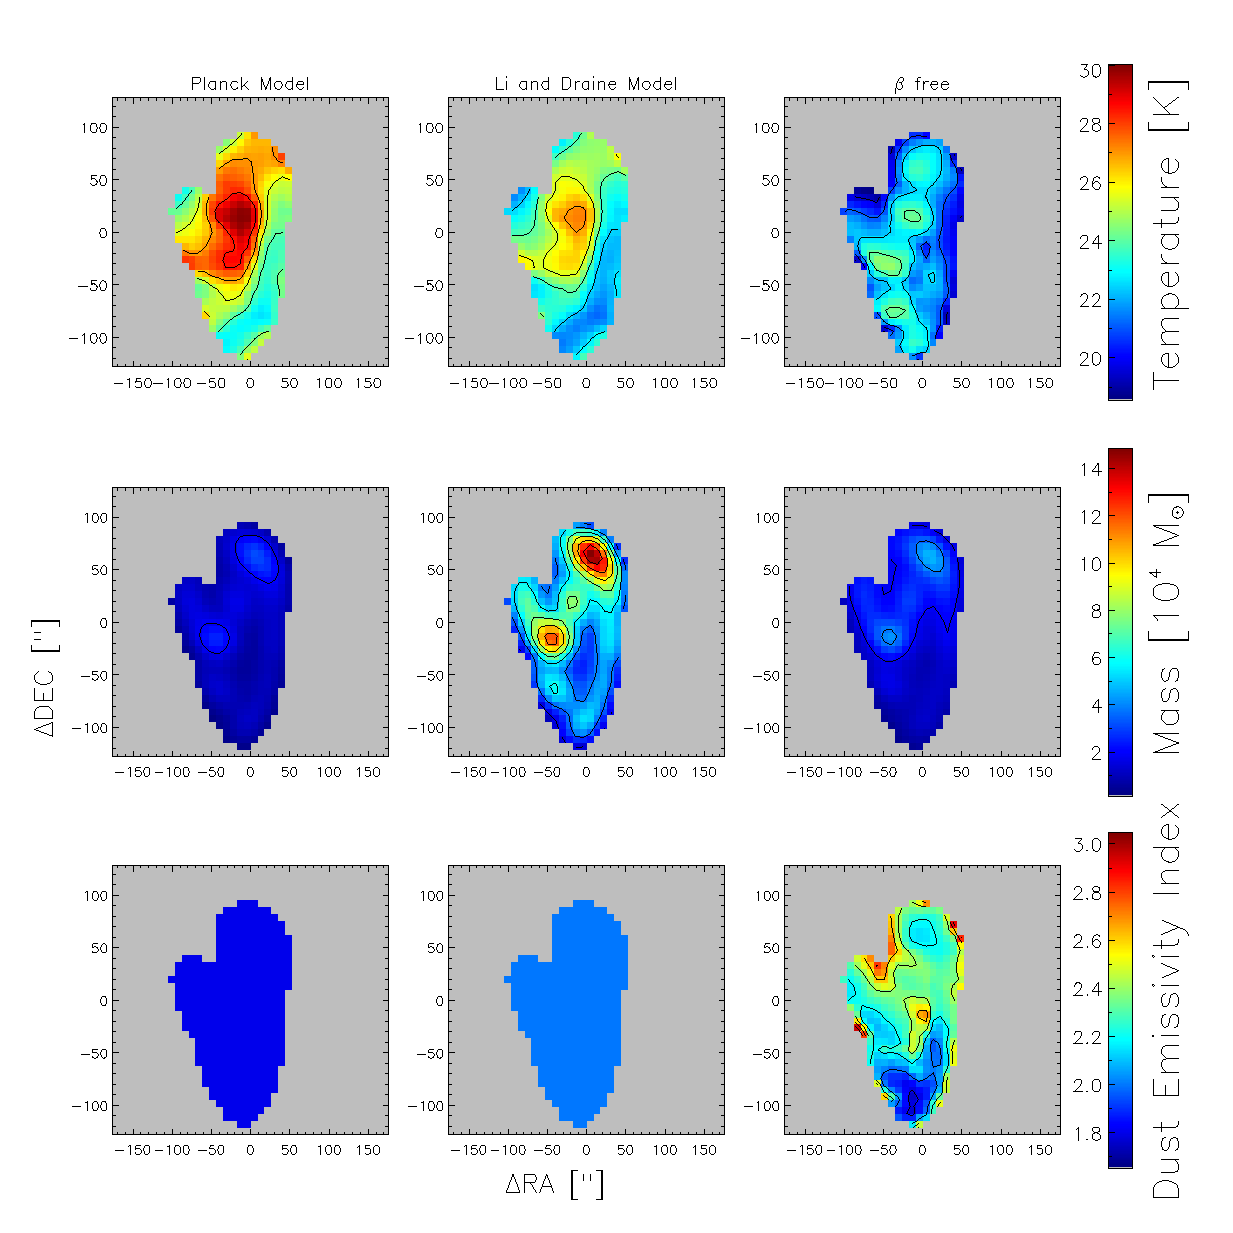
\includegraphics[width=1.\textwidth]{sed_imgs/parameter_full.eps}
  \caption[SED Parameter Maps]{Returned value for the SED fits with the Planck model in the left column, the Li and Draine model  in the middle column, and $\beta$ as a free variable in the right column.  The top row shows the temperature with contours from 1.5K to 28.5K in 1.5K increments.  The second row show the returned masses with contours from 1.9M$_\odot$ to 13.3M$_\odot$ in 1.9M$_\odot$ increments.  The bottom row shows the returned dust emissivity index values with contours from 1.8 to 2.8 with 0.2 increments.}
  \label{fig:param_fits}
\end{figure}

\begin{deluxetable}{ccccc}
  \tablecolumns{5}
  \tablewidth{0pt}
  \tablecaption{Best Fit Parameters for Planck Model}\label{tab:beta_1}
  \tablehead{\colhead{Region} & \colhead{Average $\beta$} & \colhead{ Total Mass} & \colhead{Surface Density} & \colhead{Average Temperature} \\ & &  $\left[M_\odot\right]$ & $\left[M_\odot pc^{-2}\right]$ &[K]}
  \startdata
    1 & 1.8 & 46  $\pm$ 21  & 0.09 $\pm$ 0.04 & 26   $\pm$ 2   \\
    2 & 1.8 & 11  $\pm$ 4   & 0.11 $\pm$ 0.04 & 27   $\pm$ 1   \\
    3 & 1.8 & 5.5 $\pm$ 0.9 & 0.10 $\pm$ 0.02 & 29.0 $\pm$ 0.6 \\
    4 & 1.8 & 14  $\pm$ 5   & 0.13 $\pm$ 0.05 & 27   $\pm$ 1   \\
    5 & 1.8 & 9   $\pm$ 2   & 0.07 $\pm$ 0.02 & 24   $\pm$ 1   \\
    6 & 1.8 & 3.8 $\pm$ 0.9 & 0.07 $\pm$ 0.02 & 25   $\pm$ 1   \\
  \enddata
\end{deluxetable}

\begin{deluxetable}{ccccc}
  \tablecolumns{5}
  \tablewidth{0pt}
  \tablecaption{Best Fit Parameters for Li and Draine Model}\label{tab:beta_2}
  \tablehead{\colhead{Region} & \colhead{Average $\beta$} & \colhead{ Total Mass} & \colhead{Surface Density} & \colhead{Average Temperature} \\ & &  $\left[M_\odot\right]$ & $\left[M_\odot pc^{-2}\right]$ &[K]}
  \startdata
    1 & 2.0 & 215 $\pm$ 100 & 0.11 $\pm$ 0.05 & 24   $\pm$ 2   \\
    2 & 2.0 & 53  $\pm$ 18  & 0.14 $\pm$ 0.05 & 25   $\pm$ 1   \\
    3 & 2.0 & 25  $\pm$ 4   & 0.13 $\pm$ 0.02 & 26.5 $\pm$ 0.5 \\
    4 & 2.0 & 65  $\pm$ 22  & 0.17 $\pm$ 0.06 & 24.5 $\pm$ 0.8 \\
    5 & 2.0 & 40  $\pm$ 9   & 0.09 $\pm$ 0.02 & 22.4 $\pm$ 0.9 \\
    6 & 2.0 & 17  $\pm$ 4  & 0.09 $\pm$ 0.02 & 23.5 $\pm$ 0.9 \\
  \enddata
\end{deluxetable}

\begin{deluxetable}{ccccc}
  \tablecolumns{5}
  \tablewidth{0pt}
  \tablecaption{Best Fit Parameters for $\beta$ As A Free Parameter}\label{tab:beta_f}
  \tablehead{\colhead{Region} & \colhead{Average $\beta$} & \colhead{ Total Mass} & \colhead{Surface Density} & \colhead{Average Temperature} \\ & &  $\left[M_\odot\right]$ & $\left[M_\odot pc^{-2}\right]$ &[K]}
  \startdata
    1 & 2.3  $\pm$ 0.2  & 75 $\pm$ 35 & 0.15 $\pm$ 0.07 & 22   $\pm$ 1   \\
    2 & 2.3  $\pm$ 0.2  & 19 $\pm$ 6  & 0.18 $\pm$ 0.06 & 22   $\pm$ 1   \\
    3 & 2.40 $\pm$ 0.07 & 10 $\pm$ 1  & 0.18 $\pm$ 0.03 & 23.0 $\pm$ 0.8 \\
    4 & 2.3  $\pm$ 0.1  & 23 $\pm$ 6  & 0.22 $\pm$ 0.06 & 22   $\pm$ 1   \\
    5 & 2.1  $\pm$ 0.2  & 12 $\pm$ 4  & 0.10 $\pm$ 0.03 & 22   $\pm$ 1   \\
    6 & 2.1  $\pm$ 0.1  & 5  $\pm$ 1  & 0.09 $\pm$ 0.02 & 23.0 $\pm$ 0.9 \\
  \enddata
\end{deluxetable}

%write up showing the behavior of the fits use this to segue into showing the unreliability of the 450um.  Check dates around may 5th for plots.

\subsection{Total Region Flux SED Fits}

